\documentclass[10pt, a4paper]{article}

\usepackage{xeCJK}
\usepackage{xpinyin}
\usepackage{titlesec}
%\setmainfont{Courier New}
\xpinyinsetup{ratio = 0.7}
%\setCJKmainfont{SimSun}
\usepackage[left=0.5in, right=0.5in, top=0.5in, bottom=0.5in]{geometry}
\linespread{2.4}
\renewcommand\thesubsection{\arabic{subsection}}
\titleformat{\section}{\centering\Huge}{}{0pt}{}
\titleformat{\subsection}{\centering\Huge}{\arabic{subsection}}{0pt}{}
\titlespacing{\section}{0pt}{-7ex}{-7ex}
\titlespacing{\subsection}{0pt}{-3ex}{-3ex}
\usepackage{tikz}
\usetikzlibrary{
decorations.pathmorphing,
angles,arrows,backgrounds,calc,fit,graphs,intersections,mindmap,petri,positioning,quotes,shapes,through}
\begin{document}
\section{知识回顾}
\subsection{看拼音,写汉字}
\begin{center}
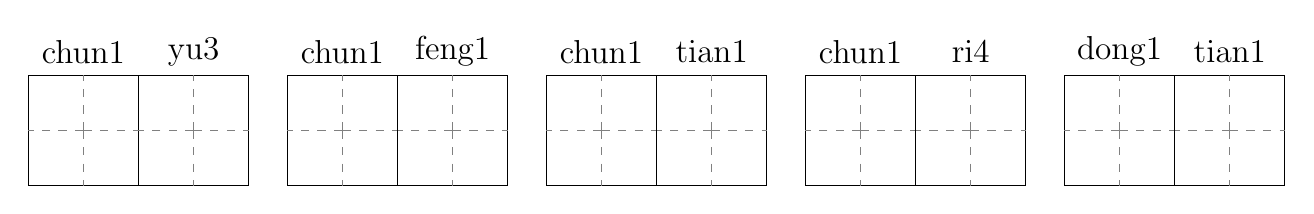
\begin{tikzpicture}
\coordinate (A) at ( 0 ,0);
\coordinate (B) at ( 1.4 ,0);
\coordinate (C) at ( 2.8 + 0.49,0);
\coordinate (D) at ( 4.2 + 0.49,0);
\coordinate (E) at ( 5.6 + 0.98,0);
\coordinate (F) at ( 7.0 + 0.98,0);
\coordinate (G) at ( 8.4 + 1.47,0);
\coordinate (H) at ( 9.8 + 1.47,0);
\coordinate (I) at (11.2 + 1.96,0);
\coordinate (J) at (12.6 + 1.96,0);
\draw (A) ++ (0, 1) node{\large\pinyin{chun1}};
\draw (B) ++ (0, 1) node{\large\pinyin{yu3}};
\draw (C) ++ (0, 1) node{\large\pinyin{chun1}};
\draw (D) ++ (0, 1) node{\large\pinyin{feng1}};
\draw (E) ++ (0, 1) node{\large\pinyin{chun1}};
\draw (F) ++ (0, 1) node{\large\pinyin{tian1}};
\draw (G) ++ (0, 1) node{\large\pinyin{chun1}};
\draw (H) ++ (0, 1) node{\large\pinyin{ri4}};
\draw (I) ++ (0, 1) node{\large\pinyin{dong1}};
\draw (J) ++ (0, 1) node{\large\pinyin{tian1}};
\foreach \P in {A,B,C,D,E,F,G,H,I,J}
{
\draw (\P) ++ (-0.7,-0.7) rectangle ++ (1.4,1.4);
\draw[dashed,gray](\P) -- +(-0.7,0 );
\draw[dashed,gray](\P) -- +(+0.7,0 );
\draw[dashed,gray](\P) -- +( 0,-0.7);
\draw[dashed,gray](\P) -- +( 0,+0.7);
}
\end{tikzpicture}
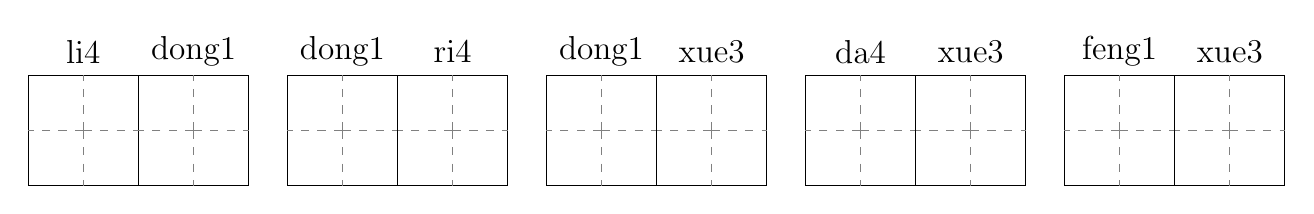
\begin{tikzpicture}
\coordinate (A) at ( 0 ,0);
\coordinate (B) at ( 1.4 ,0);
\coordinate (C) at ( 2.8 + 0.49,0);
\coordinate (D) at ( 4.2 + 0.49,0);
\coordinate (E) at ( 5.6 + 0.98,0);
\coordinate (F) at ( 7.0 + 0.98,0);
\coordinate (G) at ( 8.4 + 1.47,0);
\coordinate (H) at ( 9.8 + 1.47,0);
\coordinate (I) at (11.2 + 1.96,0);
\coordinate (J) at (12.6 + 1.96,0);
\draw (A) ++ (0, 1) node{\large\pinyin{li4}};
\draw (B) ++ (0, 1) node{\large\pinyin{dong1}};
\draw (C) ++ (0, 1) node{\large\pinyin{dong1}};
\draw (D) ++ (0, 1) node{\large\pinyin{ri4}};
\draw (E) ++ (0, 1) node{\large\pinyin{dong1}};
\draw (F) ++ (0, 1) node{\large\pinyin{xue3}};
\draw (G) ++ (0, 1) node{\large\pinyin{da4}};
\draw (H) ++ (0, 1) node{\large\pinyin{xue3}};
\draw (I) ++ (0, 1) node{\large\pinyin{feng1}};
\draw (J) ++ (0, 1) node{\large\pinyin{xue3}};

\foreach \P in {A,B,C,D,E,F,G,H,I,J}
{
\draw (\P) ++ (-0.7,-0.7) rectangle ++ (1.4,1.4);
\draw[dashed,gray]	(\P) -- +(-0.7,0 );
\draw[dashed,gray]	(\P) -- +(+0.7,0 );
\draw[dashed,gray]	(\P) -- +( 0,-0.7);
\draw[dashed,gray]	(\P) -- +( 0,+0.7);
}

\end{tikzpicture}
\end{center}
\end{document}
